\chapter{External Materials}
%TODO Write this better
\begin{itemize}
    \item Libraries
    \begin{itemize}
        \item \verb|p5.js| javascript library: \url{https://p5js.org/}
        \item \verb|tone.js| javascript library: \url{https://tonejs.github.io/}
        \item \verb|Data-Tree| javascript library:
            \url{http://cchandurkar.github.io/Data-Tree/}
    \end{itemize}
    \item Other External Materials
    \begin{itemize}
        \item Some of the initial graphics code was based on notes by my
            supervisor, John Stell
        \item The code for the additive synth was based on and heavily modified
            from \url{https://github.com/ejarzo/additive-synth}
    \end{itemize}
\end{itemize}

\chapter{User Testing Materials}
\label{questionnaire}
\section{Questionnaire}
\begin{figure}[H]
    \centering
    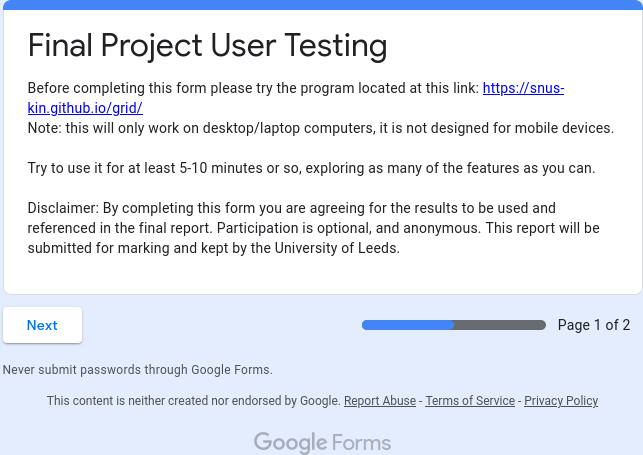
\includegraphics[width=0.7\textwidth]{quest1}
\end{figure}
\begin{figure}[H]
    \centering
    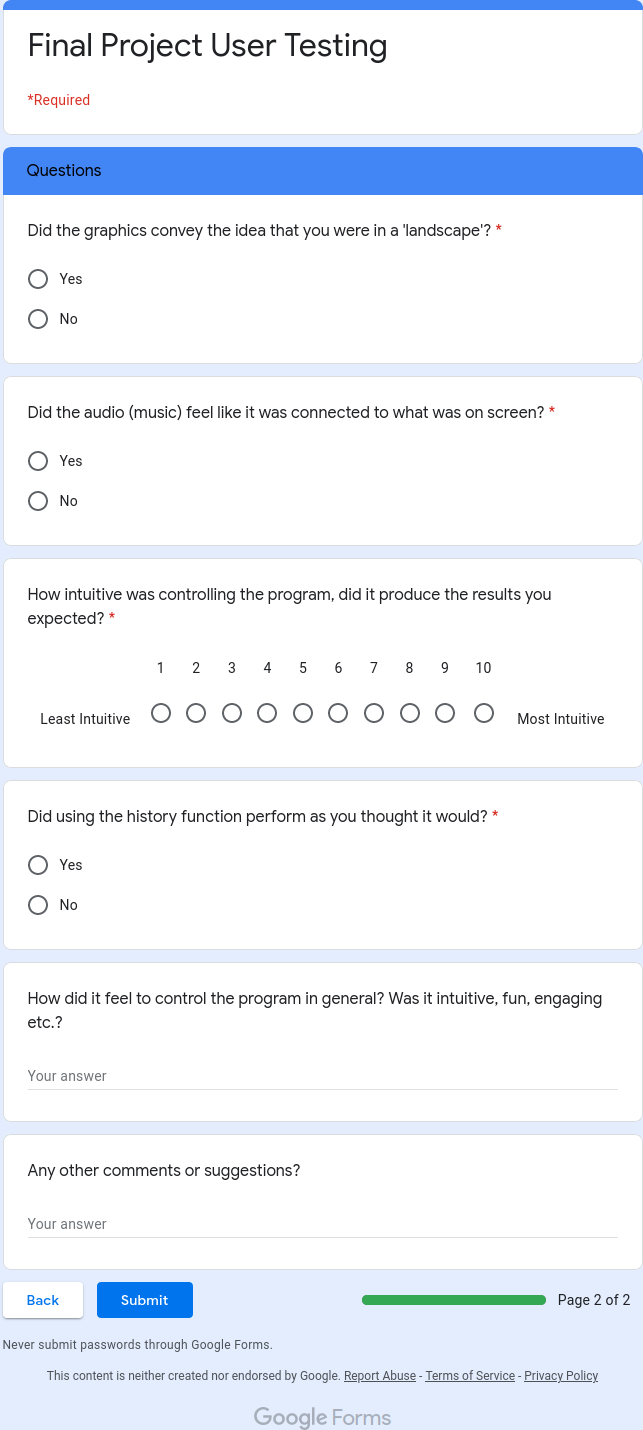
\includegraphics[width=0.5\textwidth]{quest2}
\end{figure}
\section{Results}
\subsection{Restricted Response}
\begin{figure}[H]
    \centering
    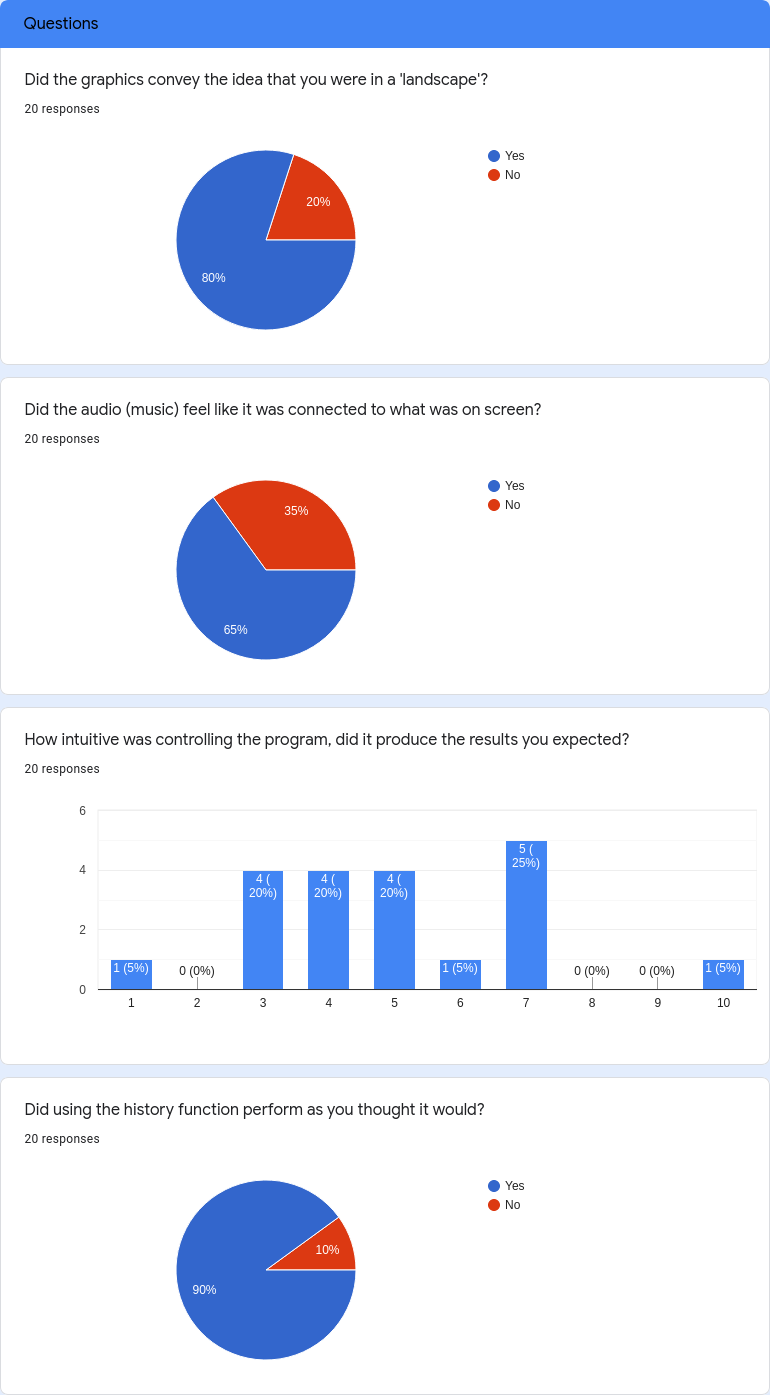
\includegraphics[width=0.7\textwidth]{usertestingresults}
\end{figure}

\subsection{How did it feel to control the program in general? Was it intuitive, fun, engaging etc.?}
\begin{itemize}
    \item Nice watching everything transform, I think it's good that you added the option
        to zoom in and out as it creates really interesting effects in terms of how the
        shapes overlap and move with each other in their wave-like clusters. The music
        is great, very immersive, makes me think of 90s Brian Eno quite a bit.

    \item All in all, an enjoyably evocative and surreal experience. The music was very
        pleasingly eerie

    \item I found it unintuitive at first but I think that was made it engaging at first.
        If I felt like I knew how it worked straight away I wouldn't have played with it
        for as long. I felt like it was a puzzle. 

    \item was a bit confusing at first, but I got a hang of it after a minute or so

    \item A little difficult to use the arrow keys, also the low sensitivity of the keys
        made it seem a little laggy in response. The sound response was exciting but it
        wasn't completely clear how movement was influencing it. 

    \item It was really neat, could definitely see myself trekking across a landscape as
        the polygons warped and shifted. A really hypnotizing experience. Love the
        musical choices as well.

    \item it was not initially clear what anything did, but after repeatedly consulting
        the controls I could explore a bit

    \item It was fascinating, a very interesting interactive project. It was simple and
        rewarding to explore the landscape.

    \item needs more labels on the buttons and more dramatic / quick change upon doing
        things. keyboard navigation was glacial

    \item It was pretty fun once i got it going but it took some time for the controls to
        have any effect - very slow movement at first

    \item Once I decided to ignore the descriptions of the controls, and sought to come up
        with my own names for them, it began to be intuitive. The discovery of the
        landscape-nature was quite interesting, and the experience was overall
        enjoyable.

    \item It would be easier if the controls were always visible. I didn't understand how
        to use it until I opened the help menu, and I wasn't able to clearly remember
        the options. I can get a sense of the controls after a while, but it's hard to
        notice immediate effects after the initial state.

    \item fun

    \item Controls were smooth. Maybe make spacing up/down a bit faster? 

    \item I felt like the changes were too slow to notice them. It was not intuitive but
        it was fun

    \item The layout of the keys was a little confusing to me, and it wasn't clear why
        some squares moved but not others -- even when I turned the randomness down,
        they seemed to still move randomly but more slowly. I liked the tree branching,
        and the overall effect is very pretty and calming.

    \item Once the controls were down, it was fun to play around with.

    \item it was cool once i got it into a state where WASDing around really changed the
        landscape yea actually i just left this open for like 45 mins zoning out to the noise
\end{itemize}

\subsection{Any other comments or suggestions?}
\begin{itemize}
    \item I found myself wanting to decide when a node on the tree was created,
        rather than have this happen automatically. I didn't use the
        upload/download features.

    \item Using the mouse for some input may feel more natural, it is hard to
        remember what keys do what, etc. The sound also stopped at some point.

    \item i couldnt read the help text, since it overflowed off the bottom of
        the screen (1366x768). personally i would rather the help button was a
        toggle rather than a hover at first glance i didnt know what the two
        arrow buttons do. best to say what they are, since when i clicked the
        down button i was interrupted by a download dialogue the UI doesnt scale
        properly with zoom, since they are positioned absolutely at load rather
        than using position: relative and letting the browser place them doesnt
        work great with browser vim plugins. but that's my fault ;)

    \item 1. Should probably by default limit what backup uploaded by users, it
        asks for all files when it just needs json. 2. History can extend past
        edge of screen and cannot be obtained once it does. Should make it
        scrollable if possible. 3. The instructions are fantastic, love the
        aesthetic and everything is clear and concise. However intuitively it
        would be nice to just click the help button to show and hide the
        instructions instead of moving the mouse over to the edge past the
        render. Otherwise, a really great art piece, loved playing around with
        it.

    \item I felt like the encoding of the landscape as shapes that slowly move
        to reflect some underlying state made it difficult to know what sort of
        movement was occurring. Before consulting the help menu, and even for a
        bit after, I interpreted the controls as manipulating the shapes rather
        than as moving around a landscape viewed through the shapes.

    \item Having an AZERTY keyboard, I had to change the keyboard to QWERTY to
        use the program. Not very important but something to consider for online
        works.

    \item didn't actually find the history function but the question was
        mandatory

    \item Sound didn't work for me :(

    \item The "history" tree on the left goes off-screen if one carries on too
        long, and becomes inaccessible, unfortunately. Perhaps a scroll
        function? (On Chrome, if that helps.)

    \item The music only seems to play in Firefox.

    \item lol funny volume button

    \item I couldn't actually hear any music, so I don't know what it was
        supposed to sound like. I had my volume up and messed with the slider
        and mute button, but nothing happened for me.

    \item lacking some "affordances" (ux term), i get you're going for artsy
        look font, favicon
\end{itemize}

\chapter{Audio Demo}
\label{audiodemo}
\begin{lstlisting}[language=java]
import processing.sound.*;

SinOsc base;
SinOsc variable;
float baseFreq = 440;
// they are in unity to start with
float variableFreq = 440;

float volume = 0.2;
float s_x,s_y,x,y = 0;
float interval;

boolean isUp, isDown, isLeft, isRight;

void settings() {
  size(501, 501);
}

void setup() {  
  base = new SinOsc(this);
  base.play();
  base.freq(baseFreq);
  base.amp(volume);

  variable = new SinOsc(this);
  variable.play();
  variable.amp(volume);
}

void draw() {
  background(255);
  translate(width/2, height/2);
  scale(1, -1);

  // make some axes
  stroke(0);
  strokeWeight(1);
  line(0,height/2,0,-height/2);
  line(width/2,0,-height,0);

  strokeWeight(4);
  point(x,y);

  // mark where the integer values will be, for demo reasons
  stroke(255,0,0);
  strokeWeight(4);
  for(int i = -3; i <= 3; i++) {
    for(int j = -3; j <= 3; j++) {
      point(map(i, -3, 3, -width/2, width/2),
            map(j, -3, 3, -height/2, height/2));
    }
  }

  // scale x and y to some reasonable numbers -3 -> 3 
  s_x = map(x, -width/2, width/2, -3, 3);
  s_y = map(y, -height/2, height/2, -3, 3);
  // now we need to find a way to scale until 
  // we're in the same octave
  interval = pow(3,s_x) * pow(5,s_y);
  
  while (interval < 1 || interval >= 2) {
    if (interval < 1) {
      interval = interval * 2;
    } else if (interval > 2) {
      interval = interval / 2;
    }
  }

  variableFreq = interval * baseFreq;
  variable.freq(variableFreq);

  if (isUp) y++;
  if (isDown) y--;
  if (isRight) x++;
  if (isLeft) x--;
}

void keyPressed() {
  setMove(key, true);
}

void keyReleased() {
  setMove(key, false);
}

void setMove(char k, boolean b) {
  if (key == 'w') isUp = b;
  if (key == 's') isDown = b;
  if (key == 'a') isLeft = b;
  if (key == 'd') isRight = b;
}
\end{lstlisting}

